\section{Passports}

The standard protocol for machine-readable travel documents is Document 9309
issued by the International Civil Aviation Organization. Since all countries
must operate on shared standard, it is necessary to forge a compromise between
cultural openness and international security. The ICAO-9309 standard gives
significant flexibility to the inclusion of national characters.

The passport data page is divided into two sections: the Visual Inspection Zone
(VIZ) and the Machine Readable Zone (MRZ). Countries may fill the required
fields of the VIZ however they desire in the national language, provided a
transcription or translation is also provided into English, Spanish, or French.
Thus compliant passports do not per se coax a country toward the adoption of
standard alphabets while still allowing international cooperation.

In the Machine Readable Zone, a transcription into the organization's approved
ASCII subset (0-9, A-Z, <) is required, for the purpose of machine recognition.
For Latin alphabet languages, most characters containing diacritics simply have
the mark dropped, although some characters have recommended control sequences to
losslessly transliterate the character. The document spells out a more extensive
scheme for Cyrilic and Arabic characters which allows nearly lossless recovery
of the original form from the highly schematic MRZ specification. There is even
a sample Python program for converting from the MRZ to Unicode Arabic.

\subsection{Latin}

In the ICAO's recommendation, a distinction is made regarding the relative
salience of diacritical marks; those such as the acute or grave accents over
vowels are simply eliminated in the MRZ. However, they provide methods of
encoding more salient characters such as the German umlaut vowels (ä,ö,ü) or the
Spanish tilde ñ.

So the name "Térèsa Cañón" would become CANXXON<<TERESA in the MRZ. Likewise,
"Wilhelm Furtwängler" would become FURTWAENGLER<<WILHELM. (b.4.2) It would not
be difficult to expand the escape sequence system in order to represent
additional diacritical marks.

\subsection{Cyrillic}

The ICAO transcription system permits a one-to-one transcription between the
machine-readable representation and the original language. The system even
recognizes the different values that a Cyrillic glyph might take in various
languages. For example the letter Ю is transliterated as "IU", unless it is the
first character of a Ukrainian name, in which case "YU" is permitted. Likewise
for Щ; this is SHCH, except in Bulgarian, where it is SHT.

\subsection{Arabic}

For example, the Arabic name

\arfont{
ابو بکر محمد بن زکریا الرازی
}

\rmfamily
would be rendered in the MRZ as:

ABW<BKR<MXHMD<<BN<ZKRYA<ALRAZY

While this looks almost incomprehensible when read by a human, the use of X as
an escape character allows a one-to-one transliteration back into the original
script. More examples below:

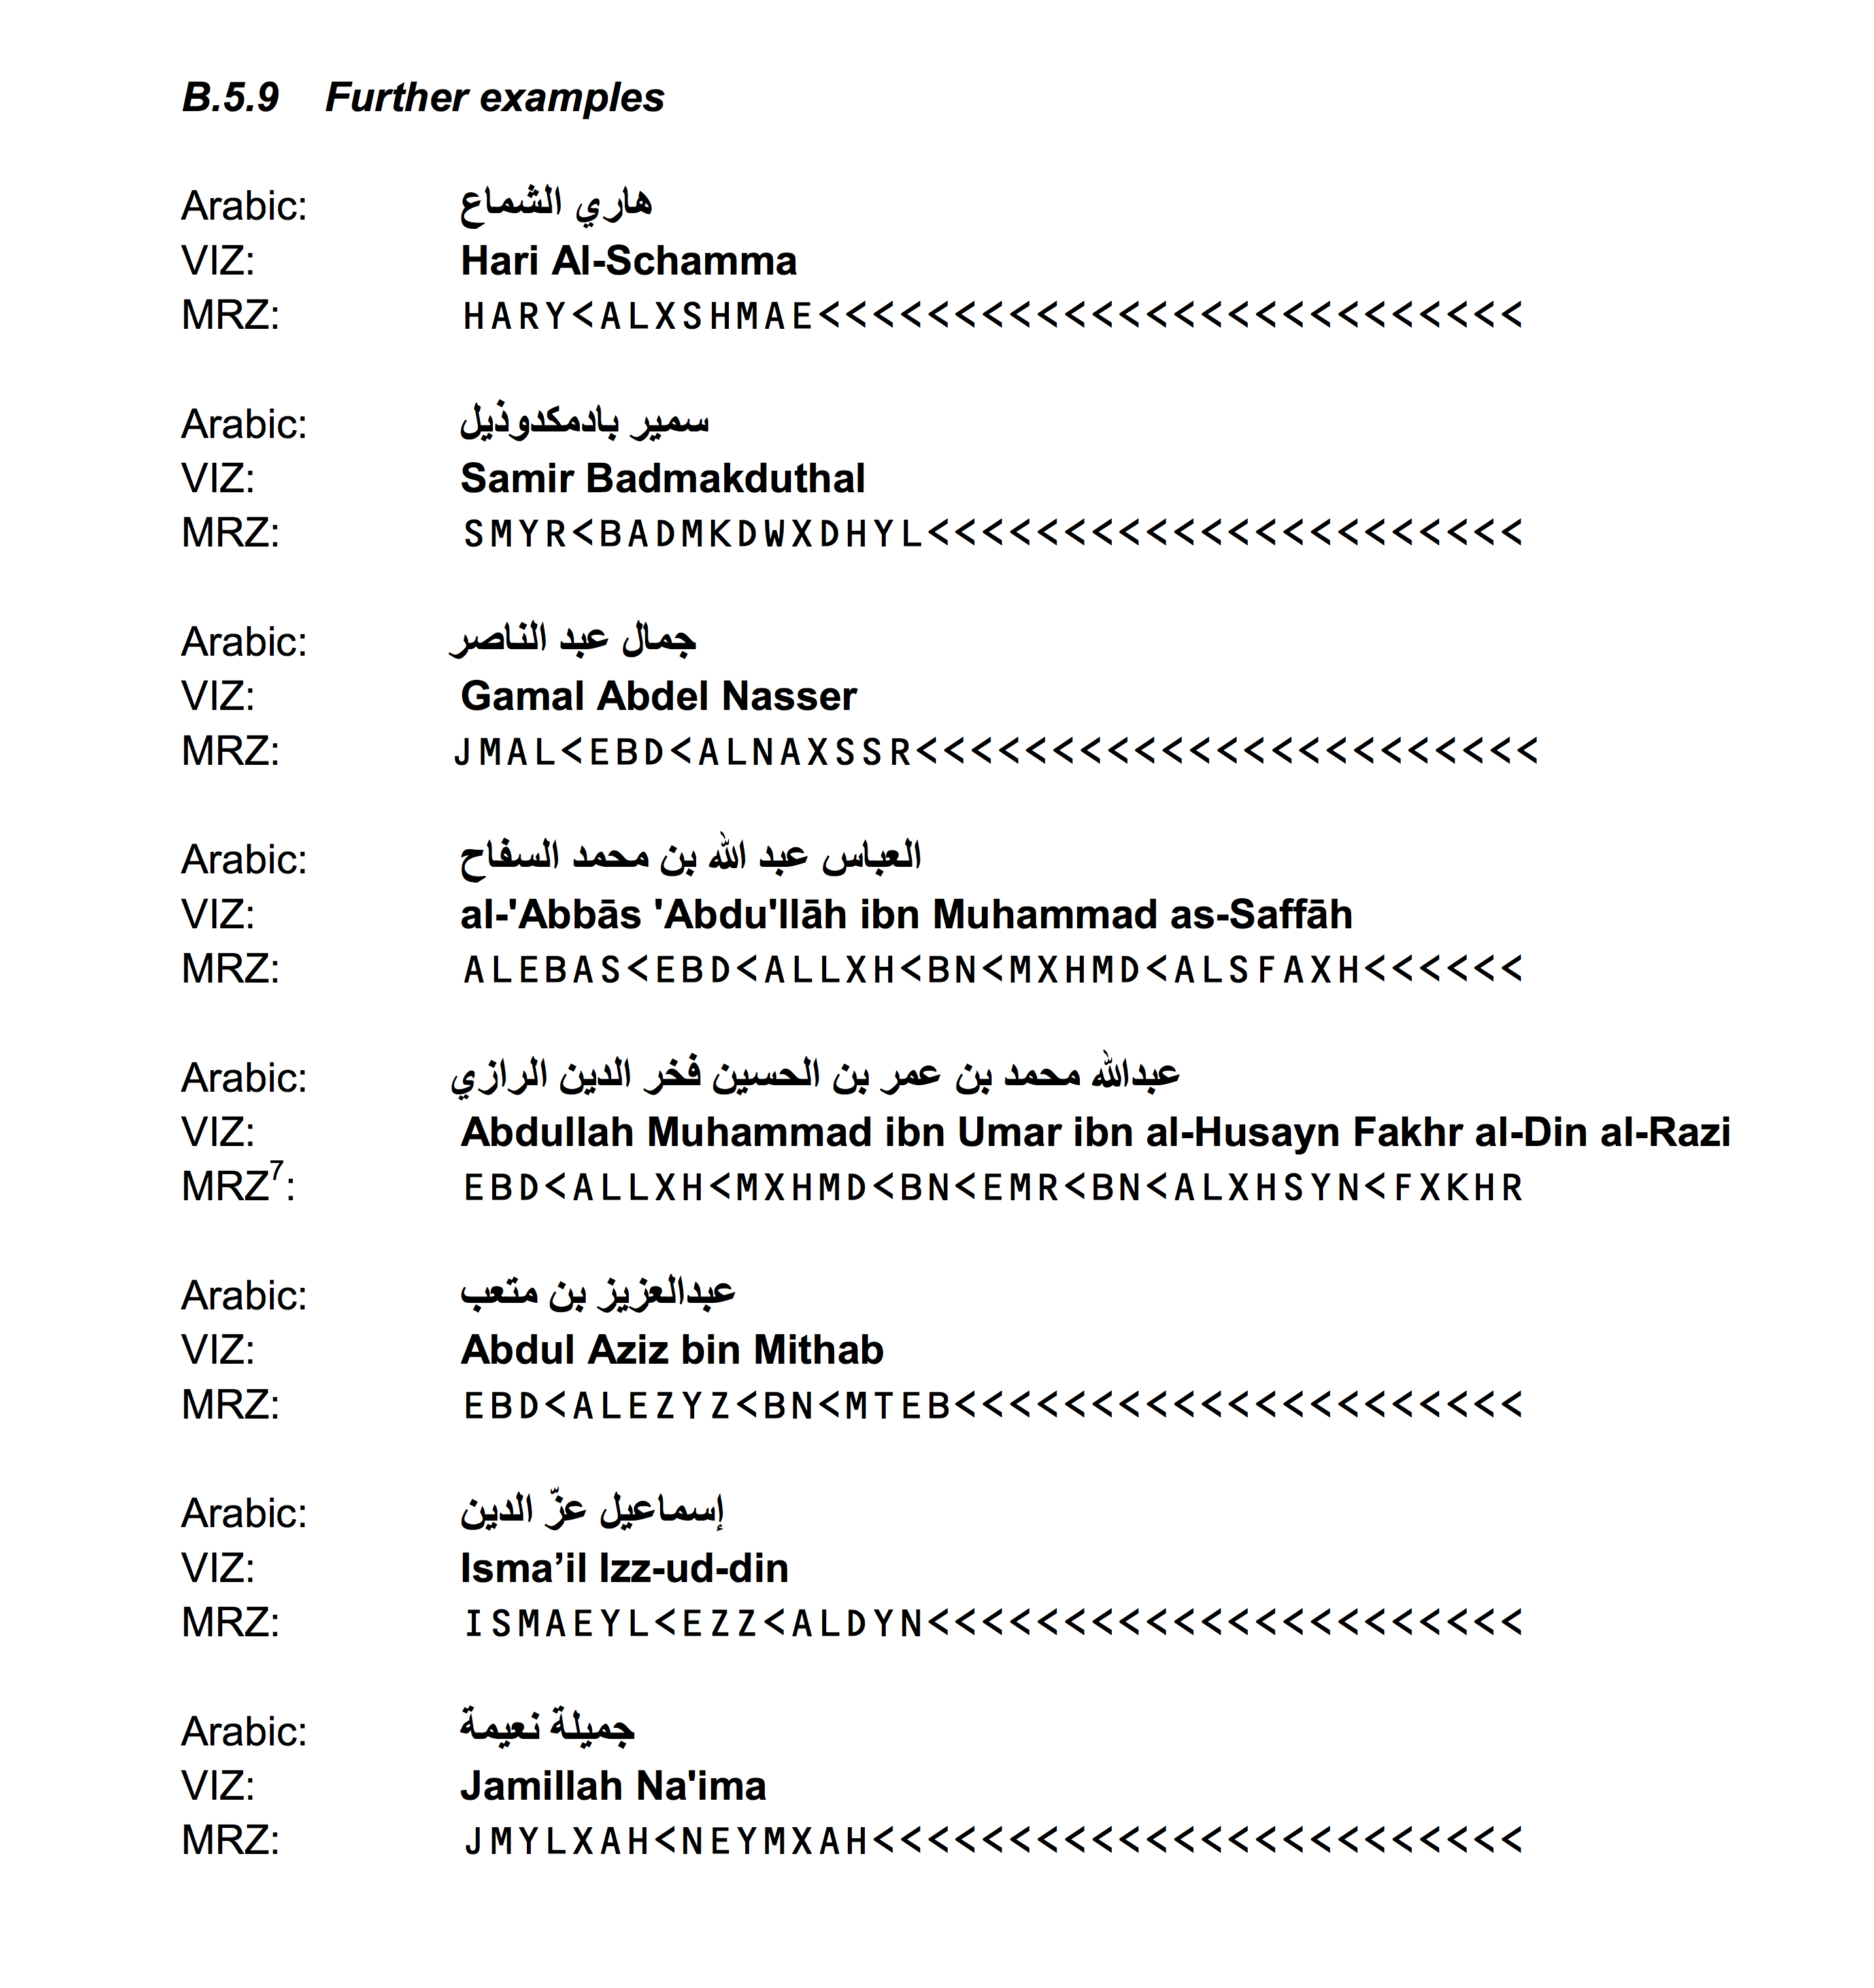
\includegraphics{../Articles/9309.3-appendix-b.5.9.png}

